\documentclass{beamer}
\usepackage[utf8]{inputenc}
\usepackage[T1]{fontenc}
\usepackage{fancyvrb}
\title{Deep Learning on the IMDB Dataset}
\date{WASP Deep Learning}
\author[Agents 47]{The Hitmen --- Agents 47}

\usetheme{wasp}

\graphicspath{{./graphics/}}

\begin{document}

\begin{frame}
  \titlepage
\end{frame}


\begin{frame}{Convnets}{Convolutional Neural Networks}

  \begin{itemize}

  \item[Training] Using all data, we reached the best result after around 1 or 2
    epochs to around 93.5 \%. By using less, say 20 \% of the data, training
    improved for up to 4 epochs, but the validation results were considerably
    worse (73 \%). Note however that training with less data is considerably
    faster.

  \item[Batch] Smaller batches train slightly faster, but doesn't otherwise
    affect validation results much (Got 94.1 \% with batch size 64). Too big
    batches may however consume too much memory for efficient training.

  \item[Reviews/Unique] Increasing these values can add a significant amount of
    data to the model, and thus \textbf{might} improve the result (93.7 \%), but
    will also take longer to train. Reducing it barely changs the result. (93.1
    \%).

  \item[Dropout] 20\% dropout helps slightly: 94.7 \%.  40\% dropout helps a bit
    more: 95.5 \%. Even higher (80 \%) didn't improve the final result, but did
    make the learning process improve for all 10 epochs.

  \item[Architecture] Krohn's architecture seems to perform slightly better, but
    takes a little longer to train than Chollet's. Comparing this with a network
    architecture with only dense layers (~88 \%), convolutional architectures seem
    superior.

  \item[Smaller Network]

  \end{itemize}

\end{frame}


\begin{frame}{Convnets}{Training History}

  \begin{columns}
    \begin{column}{0.5\textwidth}
      \begin{figure}[ht]
        \centering
        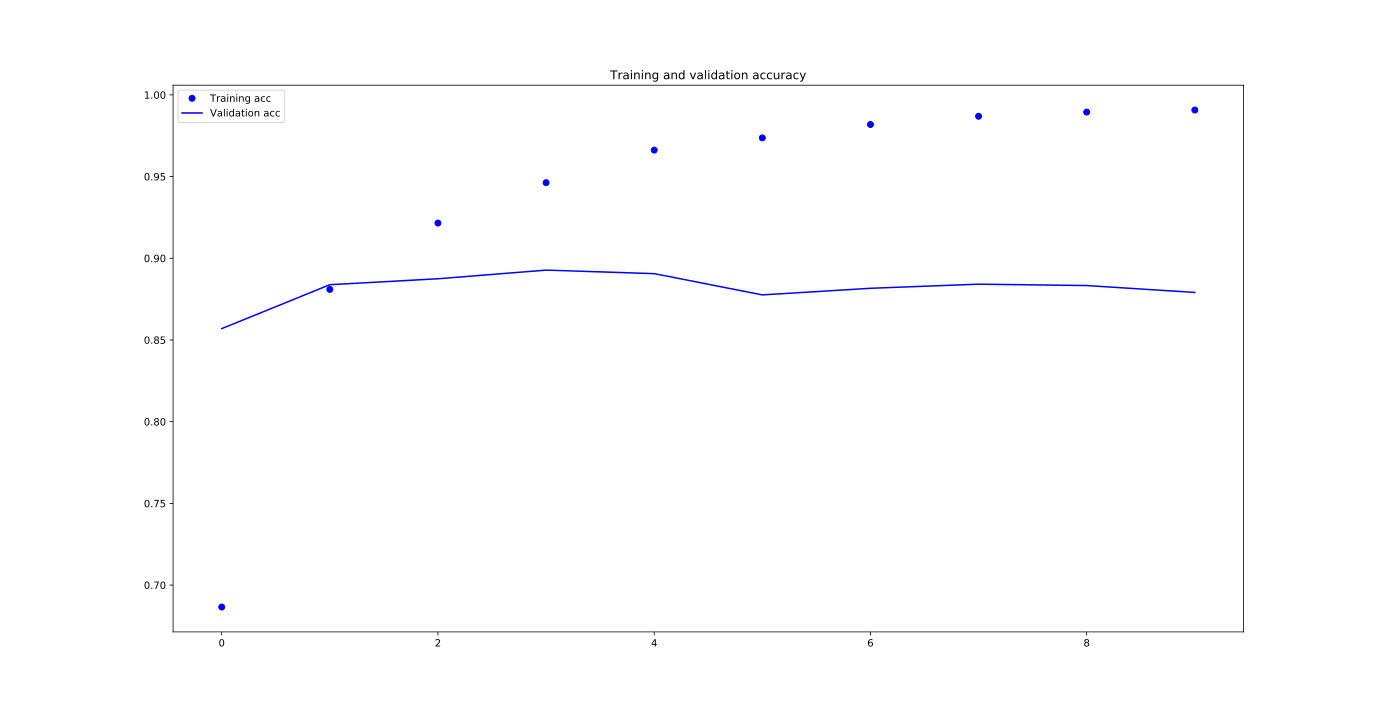
\includegraphics[width=1.2\textwidth]{convnet_training}
      \end{figure}

    \end{column}
    \begin{column}{0.5\textwidth}
      \begin{figure}[ht]
        \centering
        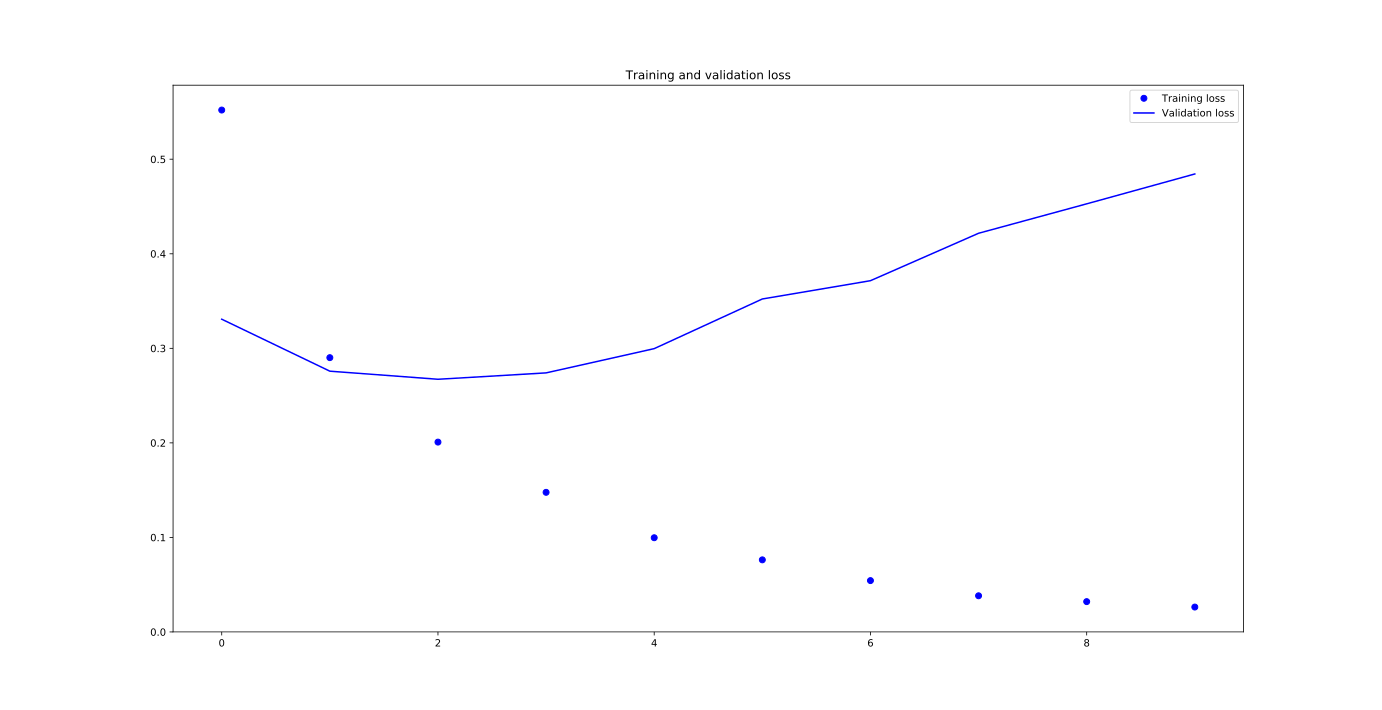
\includegraphics[width=1.2\textwidth]{convnet_loss}
      \end{figure}

    \end{column}
  \end{columns}

\end{frame}


\begin{frame}{Convnets}{Classification Confidence}

  \begin{figure}[ht]
    \centering
    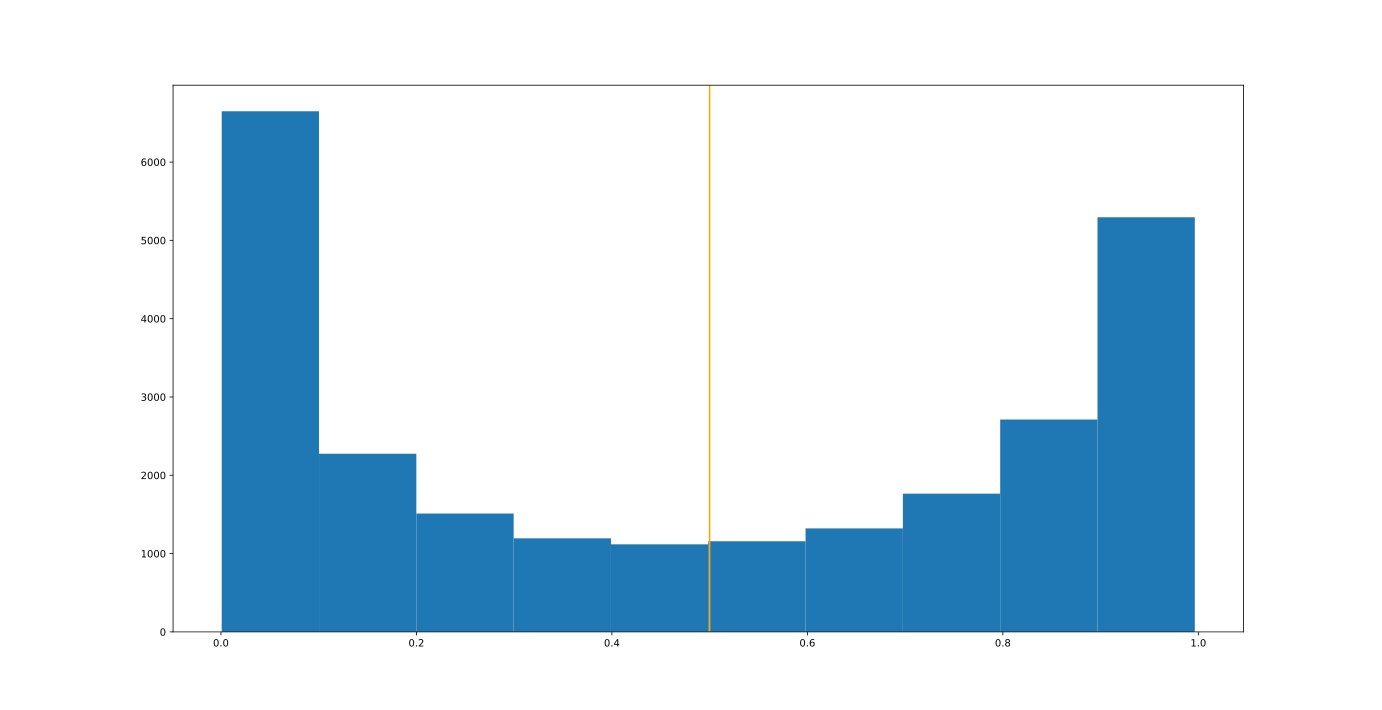
\includegraphics[width=1.0\textwidth]{convnet_histogram}
  \end{figure}

\end{frame}

\begin{frame}{Convnets}{Why Convolutions for NLP?}

  \begin{itemize}

  \item Intuitively, a 1D convolution would look both forwards and backwards in
    a sentence, mimicking how the natural language refers to earlier or coming
    words.

  \item Training for more than 1 or 2 epochs doesn't appear to be beneficial for
    classification of this data. This does however depend quite a lot on
    hyper-parameter choices.

  \end{itemize}

\end{frame}



\begin{frame}{RNN}{Recurrent Neural Networks}

\end{frame}

\begin{frame}{LSTM}{Long Short Term Memory}

\end{frame}


\begin{frame}
  \frametitle{Next Steps}
  From here, there are still a number of things one may want to do:
\end{frame}

\bgroup
\setbeamertemplate{background}{}
\setbeamercolor{background canvas}{bg=black}
% \setbeamertemplate{navigation symbols}{}
\begin{frame}[t,plain]{}{}
  \begin{center}
    {\tiny \textcolor{white}{The End}}
  \end{center}
\end{frame}
\egroup

\end{document}
